\documentclass[11pt, article, one side]{memoir}

\settrims{0pt}{0pt} % page and stock same size
\settypeblocksize{*}{34pc}{*} % {height}{width}{ratio}
\setlrmargins{*}{*}{1} % {spine}{edge}{ratio}
\setulmarginsandblock{1in}{1in}{*} % height of typeblock computed
\setheadfoot{\onelineskip}{2\onelineskip} % {headheight}{footskip}
\setheaderspaces{*}{1.5\onelineskip}{*} % {headdrop}{headsep}{ratio}
\checkandfixthelayout


%-------- Packages --------%

\usepackage{mathtools}
\usepackage{amsthm}
%\usepackage{amssymb}
\usepackage{dutchcal}
\usepackage{newpxtext}
\usepackage[varg,bigdelims]{newpxmath}
%\usepackage{eucal}
%\usepackage[usenames,dvipsnames]{xcolor}
\usepackage{tikz}
%\usepackage[siunitx]{circuitikz}
%\usepackage{graphicx}
%\usepackage{outline}
%\usepackage{varwidth}
\usepackage[inline]{enumitem}
%\usepackage{ifthen}
%\usepackage[utf8]{inputenc} %allows non-ascii in bib file
\usepackage[bookmarks=true, colorlinks=true, linkcolor=blue!50!black,
citecolor=orange!50!black, urlcolor=orange!50!black, pdfencoding=unicode]{hyperref}
\usepackage[capitalize]{cleveref}
\usepackage[backend=biber, backref=true, maxbibnames = 10, style = alphabetic]{biblatex}
%\usepackage[framemethod=tikz]{mdframed}
%\usepackage{todonotes}
\usepackage{ytableau} % for Young diagrams

%-------- Package setup --------%

% cleveref %
  \newcommand{\creflastconjunction}{, and\nobreakspace} % serial comma

% biblatex %
  \addbibresource{refs.bib} 

% makeidx %
  \makeindex 

% hyperref %
  \hypersetup{final}

% enumitem %
  \setlist{nosep}
  

% tikz %
  \usetikzlibrary{ 
  	cd,
  	math,
  	decorations.markings,
  	decorations.pathmorphing,
		decorations.pathreplacing,
  	positioning,
  	arrows.meta,
  	shapes,
		shadows,
		shadings,
  	calc,
  	fit,
  	quotes,
  	intersections,
    circuits,
    circuits.ee.IEC
  }
  
	\tikzcdset{arrow style=tikz, diagrams={>=To}}

% mdframed/tablefootnote%
% This makes \tablefootnote allow construction of footnotes that appear at bottom of page instead of inside frame


%\mdfdefinestyle{exerciseframe}{
%    linecolor=white!93!yellow,
%    backgroundcolor=white!93!yellow,
%    }


% amsthm %
  \theoremstyle{theorem}
  \newtheorem{theorem}[section]{Theorem}
  \newtheorem{proposition}[section]{Proposition}
  \newtheorem{corollary}[section]{Corollary}
  \newtheorem{lemma}[section]{Lemma}
  
  \theoremstyle{definition}
  \newtheorem{definition}[section]{Definition}
  \newtheorem{notation}[section]{Notation}
  \newtheorem{axiom}{Axiom}
  \newtheorem*{axiom*}{Axiom}
  
  \theoremstyle{remark}
  \newtheorem{example}[section]{Example}
  \newtheorem{remark}[section]{Remark}
  \newtheorem{warning}[section]{Warning}
%  \newtheorem{exercise}[equation]{Exercise}

% Adjunctions
\newcommand{\adj}[5][30pt]{%[size] Cat L, Left, Right, Cat R.
\begin{tikzcd}[ampersand replacement=\&, column sep=#1]
  #2\ar[r, shift left=6pt, "#3"]
    \ar[l, phantom, "\scriptstyle\bot"]\&
  #5\ar[l, shift left=6pt, "#4"]
\end{tikzcd}
}

\newcommand{\adjr}[5][30pt]{%[size] Cat R, Right, Left, Cat L.
\begin{tikzcd}[ampersand replacement=\&, column sep=#1]
  #2\ar[r, shift left=6pt, "#3"]\&
  #5\ar[l, shift left=6pt, "#4"]
  \ar[l, phantom, "\scriptstyle\top"]
\end{tikzcd}
}

  
%-------- Single symbols --------%
	
\DeclareSymbolFont{stmry}{U}{stmry}{m}{n}
\DeclareMathSymbol\fatsemi\mathop{stmry}{"23}

\DeclareFontFamily{U}{mathx}{\hyphenchar\font45}
\DeclareFontShape{U}{mathx}{m}{n}{
      <5> <6> <7> <8> <9> <10>
      <10.95> <12> <14.4> <17.28> <20.74> <24.88>
      mathx10
      }{}
\DeclareSymbolFont{mathx}{U}{mathx}{m}{n}
\DeclareFontSubstitution{U}{mathx}{m}{n}
\DeclareMathAccent{\widecheck}{0}{mathx}{"71}


%-------- Renewed commands --------%

\renewcommand{\ss}{\subseteq}

%-------- Other Macros --------%

\DeclarePairedDelimiter{\pair}{\langle}{\rangle}
\DeclarePairedDelimiter{\copair}{[}{]}
\DeclarePairedDelimiter{\floor}{\lfloor}{\rfloor}
\DeclarePairedDelimiter{\ceil}{\lceil}{\rceil}

\DeclarePairedDelimiter{\corners}{\ulcorner}{\urcorner}




\DeclareMathOperator{\Hom}{Hom}
\DeclareMathOperator{\Mor}{Mor}
\DeclareMathOperator{\dom}{dom}
\DeclareMathOperator{\cod}{cod}
\DeclareMathOperator*{\colim}{colim}
\DeclareMathOperator{\im}{im}
\DeclareMathOperator{\ob}{Ob}
\DeclareMathOperator{\Tr}{Tr}
\DeclareMathOperator{\dju}{\sqcup}
\DeclareMathOperator{\plpl}{+\!+}

\DeclareMathOperator{\const}{\mathtt{const}}

\newcommand{\Set}[1]{\mathrm{#1}}%a named set
\newcommand{\cat}[1]{\mathcal{#1}}%a generic category
\newcommand{\Cat}[1]{\mathsf{#1}}%a named category
\newcommand{\fun}[1]{\textit{#1}}%function
\newcommand{\Fun}[1]{\mathbf{#1}}%functor
\newcommand{\type}[1]{\texttt{#1}}

\newcommand{\id}{\mathrm{id}}
\newcommand{\cocolon}{:\!}
\newcommand{\iso}{\cong}
\newcommand{\too}{\longrightarrow}
\newcommand{\tto}{\rightrightarrows}
\newcommand{\To}[1]{\xrightarrow{#1}}
\newcommand{\Tto}[3][13pt]{\begin{tikzcd}[sep=#1, cramped, ampersand replacement=\&, text height=1ex, text depth=.3ex]\ar[r, shift left=2pt, "#2"]\ar[r, shift right=2pt, "#3"']\&{}\end{tikzcd}}
\newcommand{\Too}[1]{\xrightarrow{\;\;#1\;\;}}
\newcommand{\from}{\leftarrow}
\newcommand{\From}[1]{\xleftarrow{#1}}
\newcommand{\Fromm}[1]{\xleftarrow{\;\;#1\;\;}}
\newcommand{\surj}{\twoheadrightarrow}
\newcommand{\inj}{\rightarrowtail}
\newcommand{\wavyto}{\rightsquigarrow}
\newcommand{\lollipop}{\multimap}
\newcommand{\pr}{\mathrm{pr}}
\newcommand{\tickar}{\begin{tikzcd}[baseline=-0.5ex,cramped,sep=small,ampersand 
replacement=\&]{}\ar[r,tick]\&{}\end{tikzcd}}
\newcommand{\imp}{\Rightarrow}
\renewcommand{\iff}{\Leftrightarrow}
\renewcommand{\th}{\ensuremath{^\tn{th}}\ }
\newcommand{\down}{\mathbin{\downarrow}}
\newcommand{\then}{\mathbin{\scalebox{.8}{/\!\!/}}}
\newcommand{\op}{^\tn{op}}
\newcommand{\grph}[1]{{#1}_{\mathrm{Gr}}}

\newcommand{\tn}[1]{\textnormal{#1}}
\newcommand{\ol}[1]{\overline{#1}}
\newcommand{\ord}[1]{\underline{#1}}
\newcommand{\wt}[1]{\widetilde{#1}}
\newcommand{\wh}[1]{\widehat{#1}}
\newcommand{\ubar}[1]{\underaccent{\bar}{#1}}
\newcommand{\LMO}[2][over]{\ifthenelse{\equal{#1}{over}}{\overset{#2}{\bullet}}{\underset{#2}{\bullet}}}
\newcommand{\LTO}[2][\bullet]{\overset{\tn{#2}}{#1}}


\newcommand{\bb}{\mathbb{B}}
\newcommand{\nn}{\mathbb{N}}
%\newcommand{\PP}{\mathbb{P}}
\newcommand{\zz}{\mathbb{Z}}
\newcommand{\rr}{\mathbb{R}}
\newcommand{\oo}{\mathcal{O}}
\newcommand{\singleton}{\{1\}}
\newcommand{\powset}{\Fun{P}}
\newcommand{\upset}{\Fun{U}}

\newcommand{\foo}{\const{foo}}
\newcommand{\true}{\const{true}}
\newcommand{\false}{\const{false}}

\newcommand{\inv}{^{-1}}

\newcommand{\boxCD}[2][black]{\fcolorbox{#1}{white}{\begin{varwidth}{\textwidth}\centering #2\end{varwidth}}}

\newcommand{\lo}[2]{#1(\,\cdot\,)^{#2}}

\newcommand{\smset}{\Cat{Set}}
\newcommand{\smcat}{\Cat{Cat}}
\newcommand{\fin}{\Cat{Fin}}
\newcommand{\cont}{\Cat{Cont}}
\newcommand{\core}{\Fun{Core}}
\newcommand{\bun}{\Cat{Bun}}

\newcommand{\zero}[1]{#1_\text{zc}}

\newcommand{\yon}{\mathcal{y}}
\newcommand{\poly}{\Cat{Poly}}
\newcommand{\dir}{\Cat{Dir}}
\newcommand{\ff}{\mathbb{F}}
\newcommand{\mdot}{{\cdot}}

\newcommand{\qand}{\quad\text{and}\quad}
\newcommand{\qqand}{\qquad\text{and}\qquad}

\newcommand{\inote}[1]{{\color{blue}David I.\ says: #1}}
\newcommand{\jnote}[1]{{\color{red}David J.\ says: #1}}


\newcommand{\cp}{\mathbin{\fatsemi}}

%%fakesubsubsection generators
%}

\linespread{1.07}
%\allowdisplaybreaks
\setsecnumdepth{subsubsection}
\settocdepth{subsection}
\setlength{\parindent}{15pt}
\setcounter{tocdepth}{2}
\setlength{\parskip}{0em}

\begin{document}

\title{Dirichlet Polynomials form a Topos}

\author{David I.\ Spivak%
\thanks{Spivak was supported by Honeywell Inc.\ as well as AFOSR grants FA9550-17-1-0058 and FA9550-19-1-0113.}
\and David Jaz Myers%\thanks{Myers thanks}
}

\maketitle
\begin{abstract}
One can think of power series or polynomials in one variable, such as $P(\yon)=2\yon^3+\yon+5$, as functors from the category $\smset$ of sets to itself; these are known as polynomial functors. Denote by $\poly_\smset$ the category of polynomial functors on $\smset$ and natural transformations between them. The constants $0,1$ and operations $+,\times$ that occur in $P(\yon)$ are actually the initial and terminal objects and the coproduct and product in $\poly_\smset$. 

Just as the polynomial functors on $\smset$ are the copresheaves that can be written as sums of representables, one can express any Dirichlet series, e.g.\ $\sum_{n=0}^\infty n^\yon$, as a coproduct of representable presheaves. A Dirichlet polynomial is a finite Dirichlet series, that is, a finite sum of representables $n^{\yon}$. We discuss how both polynomial functors and their Dirichlet analogues can be understood in terms of bundles, and go on to prove that the category of Dirichlet polynomials is an elementary topos.

%We also show that there is a double category, useful in applications, whose vertical category is isomorphic to $\poly$ and whose horizontal category is isomorphic to $\dir$.
\end{abstract}

Polynomials $P(\yon)$ and finite Dirichlet series $D(\yon)$ in one variable $\cat{y}$, with natural number coefficients $a_i\in\nn$, are respectively functions of the form
\begin{equation}\label{eqn.poly_dir_simple}
\begin{aligned}
  P(\yon)&=a_n\yon^n+\cdots+a_2\yon^2+a_1\yon^1+a_0\yon^0,\\
  D(\yon)&=a_n n^\yon+\cdots+a_22^\yon+a_11^\yon+a_00^\yon.
\end{aligned}
\end{equation}
The first thing we should emphasize is that the algebraic expressions in \eqref{eqn.poly_dir_simple} can in fact be regarded as \emph{objects in a category}, in fact two categories: $\poly$ and $\dir$. We will explain the morphisms later, but for now we note that in $\poly$, $\yon^2=\yon\times\yon$ is a product and $2\yon=\yon+\yon$ is a coproduct, and similarly for $\dir$. The operators---in both the polynomial and the Dirichlet case---are not just algebraic, they are category-theoretic. Moreover, these categories have a rich structure. 

The category $\poly$ is well studied (see \cite{GK:Polynomial.Functors}). In particular, the following are equivalent:
\begin{theorem}{\cite{GK:Polynomial.Functors}}
For a functor $P : \finset \to \finset$, the following are equivalent:
\begin{enumerate}
    \item $P$ is polynomial.
    \item $P$ is a sum of representables.
    \item $P$ preserves connected limits -- or equivalently, wide pullbacks.
\end{enumerate}
\end{theorem}

We will prove an analogous result characterizing Dirichlet polynomials:
\begin{theorem}
For a functor $D : \finset\op \to \finset$, the following are equivalent:
\begin{enumerate}
    \item $D$ is a Dirichlet polynomial.
    \item $D$ is a sum of representables.
    \item $D$ sends connected colimits to limits -- or equivalently, $D$ preserves wide pushouts.
\end{enumerate}
\end{theorem}

We will also show that $\dir$ is equivalent to the arrow category of finite sets, 
\[\dir \simeq \fin^{\to},\]
and in particular that $\dir$ is an elementary topos.

If one allows \emph{arbitary} sums of functors represented by finite sets, one gets \emph{analytic} functors in the covariant case---first defined by Joyal in his seminal paper on combinatorial species \cite{J:Combinatorial.Species}---and \emph{Dirichlet} functors in the contravariant case---first defined by Baez and Dolan and appearing in Baez's \emph{This Week's Finds} blog \cite{BD:This.Weeks.Finds.300}. Baez and Dolan also drop the traditional negative sign in the exponent (that is, they use $n^s$ where $n^{-s}$ usually appears), but also find a nice way to bring it back by moving to groupoids. Here, we drop the negative sign and work with finite sets to keep things as simple as possible. Similar considerations hold with little extra work for infinite Dirichlet series or power series, and even more generally, by replacing $\fin$ with $\smset$. 


% While we will not belabor the point, our main goal is to make it clear that one should not generally drop the $a_0\cdot0^\yon$ term from a Dirichlet series as in \cref{eqn.poly_dir_simple}. To make the case, we will begin by defining the categories $\poly$ and $\dir$. These categories have excellent formal properties; for example we will show in \cref{cor.dir_topos} that $\dir$ is an elementary topos. In some sense the ``high status'' of the category $\dir$ is supposed to serve as evidence that identifying $0^\yon$ with the initial object $0$ could lead to perverse outcomes and thus may be fruitfully reconsidered.

\chapter{Polynomial and Dirichlet functors}

Recall that a \emph{co-representable functor} $\fin\to\fin$ is one of the form $\fin(k, -)$ for a finite set
\[k=\{`1', `2',\ldots,`k'\}.\]
We denote this functor by $\yon^k$ and say it is \emph{represented by} $k\in\fin$. Similarly, a \emph{(contra-) representable functor} $\fin\op\to\fin$ is contravariant functor of the form $\fin(-,k)$; we denote this functor by $k^\yon$. The functors $\yon^-$ and $-^\yon$ are the contravariant and covariant Yoneda embeddings,
\[
  \yon^k \coloneqq \fin(k,-)
  \qqand
  k^\yon\coloneqq\fin(-,k).
\]
For example $\yon^3(2)\cong8$ and $3^\yon(2)\cong9$.

Note that the functor $0^\yon\not\cong 0$ is not the initial object in $\dir$; it is given by
\[
0^\yon(s)=
\begin{cases}
1&\tn{ if } s=0\\
0&\tn{ if } s\geq1.
\end{cases}
\]
The coefficient $a_0$ of $1=\yon^0$ in a polynomial $P$ is called its \emph{constant} term. We refer to the coefficient $\zero{D}\coloneqq a_0$ of $0^\yon$ in a Dirichlet series $D$ as its \emph{zero-content} term. Rather than having no content, the content of the functor $\zero{D}\mdot0^\yon$ becomes significant exactly when it is applied to zero.

\begin{example}
The reader can determine which finite Dirichlet series $D(\yon)$ as in \cref{eqn.poly_dir_simple} has the following terms
\[
\begin{array}{c|ccccccc}
\yon&
\cdots&
5&
4&
3&
2&
1&
0
\\\hline
D(\yon)&
\cdots&
96&
48&
24&
12&
6&
7
\end{array}
\]
Hint: its zero-content term is $\zero{D}=4$.
\end{example}

The set $P(1)$ (resp.\ the set $D(0)$) has particular importance; it is the set of pure-power terms $\yon^k$ in $P$ (resp.\ the pure-exponential terms $k^\yon$ in $D$). For example if $P=\yon^2+4\yon+4$ and $D=2^\yon+4+4\mdot0^\yon$ then $P(1)=D(0)=9$. We will later have reason to consider the inclusion
\begin{equation}\label{eqn.zerocontent}
\zero{D}\to D(0)
\end{equation}
of the zero-content terms into the set of all pure-exponential terms.

\begin{definition}\label{def.poly_dir_obs}
A \emph{polynomial functor} is a functor $P\colon\fin\to\fin$ that can be expressed as a sum of co-representable functors. Similarly, we define a \emph{Dirichlet functor} to be a functor $D\colon\fin\op\to\fin$ that can be expressed as a sum of representable presheaves (contravariant functors):
\begin{equation}\label{eqn.finite_sum}
  P=\sum_{i=1}^{P(1)}\yon^{p_i}
  \qqand
  D=\sum_{i=1}^{D(0)}(d_i)^\yon.
\end{equation}
That is, $P(X)=\sum_{i=1}^{P(1)}\fin(p_i,X)$ and $D(X)=\sum_{i=1}^{D(0)}\fin(X,d_i)$ as functors applied to $X\in\fin$.
\end{definition}

Note that \cref{def.poly_dir_obs} generalizes to any category, but it is not generally equivalent to the usual definition of polynomial functor, defined on any locally cartesian closed category; see \cite{GK:Polynomial.Functors}.

\chapter{The categories $\poly$ and $\dir$}

For any small category $C$, let $\fin^C$ denote the category whose objects are the functors $C\to\fin$ and whose morphisms are the natural transformations between them.
\begin{definition}\label{def.poly_dir}
The \emph{category of polynomial functors}, denoted $\poly$, is the full subcategory of $\fin^\fin$ spanned by sums $P$ of representable functors. The \emph{category of Dirichlet functors}, denoted $\dir$, is the full subcategory of $\fin^{(\fin\op)}$ spanned by the sums $D$ of representable presheaves.
\end{definition}

While we will not pursue it here, one can take $\poly_\smset$ to be the full subcategory of functors $\smset\to\smset$ spanned by small coproducts of representables, and similarly for $\dir_\smset$. 


\begin{lemma}\label{lemma.count_maps}
The number of polynomial maps $P\to Q$ and Dirichlet maps $D\to E$ are given by the following formulas:
\[
  \poly(P,Q)\coloneqq\prod_{i\in P(1)}Q(p_i)
  \qqand
  \dir(D,E)\coloneqq\prod_{i\in D(0)}E(d_i).
\]
\end{lemma}

\begin{example}
Let $P=2\yon^2$, $Q=\yon+1$, and let $D=2\cdot2^\yon$ and $E=1+0^\yon$. Then there are nine ($9$) polynomial morphisms $P\to Q$, zero ($0$) polynomial morphisms $Q\to P$, one ($1$) Dirichlet morphism $D\to E$, and eight ($8$) Dirichlet morphisms $E\to D$.
\end{example}

\begin{remark}\label{rem.products_coproducts}
Sums and products of polynomials in the usual algebraic sense agrees exactly with sums and products in the categorical sense: if $P$ and $Q$ are polynomials, i.e.\ objects in $\poly$, then their coproduct is $P+Q$ and their product is $PQ$. The same is true for $\dir$: sums and products of Dirichlet polynomials in the usual sense agree exactly with sums and products in the categorical sense.
\end{remark}

\paragraph{Formal structures.}
There is an adjoint quadruple and adjoint sextuple as follows, labeled by where they send objects $n\in\fin$, $P\in\poly$, $D\in\dir$:
\begin{equation}\label{eqn.adjoints_galore}
\begin{tikzcd}[column sep=60pt]
  \fin
  	\ar[r, shift left=7pt, "n" description]
		\ar[r, shift left=-21pt, "n\yon"']&
  \poly
  	\ar[l, shift right=21pt, "P(0)"']
  	\ar[l, shift right=-7pt, "P(1)" description]
	\ar[l, phantom, "\scriptstyle\top"]
	\ar[l, phantom, shift left=14pt, "\scriptstyle\top"]
	\ar[l, phantom, shift right=14pt, "\scriptstyle\top"]
\end{tikzcd}
\hspace{1in}
\begin{tikzcd}[column sep=60pt]
  \fin
  	\ar[r, shift left=7pt, "n\cdot 0^\yon" description]
		\ar[r, shift left=-21pt, "n" description]
		\ar[r, shift left=-49pt, "n^\yon"']&
  \dir
  	\ar[l, shift right=21pt, "\zero{D}"']
  	\ar[l, shift right=-7pt, "D(0)" description]
		\ar[l, shift right=-35pt, "D(1)" description]
	\ar[l, phantom, shift right=14pt, "\scriptstyle\bot"]
	\ar[l, phantom, shift right=0pt, "\scriptstyle\bot"]
	\ar[l, phantom, shift right=-14pt, "\scriptstyle\bot"]
	\ar[l, phantom, shift right=-28pt, "\scriptstyle\bot"]
	\ar[l, phantom, shift right=-42pt, "\scriptstyle\bot"]
\end{tikzcd}
\end{equation}
All six of the displayed functors out of $\fin$ are fully faithful.

The inclusion $\zero{D}\to D(0)$ from \cref{eqn.zerocontent} is natural and induces three other natural transformations on $\fin$ and $\dir$ via the adjunctions in \cref{eqn.adjoints_galore}; in \cref{prop.poly_function} we will have occasion to use the one labeled $\pi_D$:
\begin{equation}\label{eqn.obtain_pi}
\zero{D}\to D(0),\qquad
n\mdot0^\yon\to n,\qquad
D(1)\To{\pi_D} D(0),\qquad
n\to n^\yon.
\end{equation}

Polynomials functors can of course be composed $(P\circ Q)(n)\coloneqq P(Q(n))$; this gives a nonsymmetric monoidal structure on $\poly$. The monoidal unit is $\yon$.

Day convolution for the cartesian product monoidal structure provides symmetric monoidal structure $\otimes\colon\poly\times\poly\to\poly$, for which the monoidal unit is $\yon$. This monoidal structure---like the Cartesian monoidal structure---distributes over $+$ We can write an explicit formula for $P\otimes Q$, with $P,Q$ as in \cref{eqn.finite_sum}:
\begin{equation}\label{eqn.dir_monoidal_product}
  P\otimes
  Q=
  \sum_{i=1}^{P(1)}\sum_{j=1}^{Q(1)}\yon^{p_iq_j}
\end{equation}
We call this the \emph{Dirichlet product} of polynomials, for reasons we will see in \cref{rem.dir_prod_reason}.

The Dirichlet monoidal structure is closed; that is, for any $A,Q:\poly$ we define
\begin{equation}\label{eqn.poly_mon_closed}
[A,Q]\coloneqq\prod_{i:A(1)}Q\circ(a_i\yon),
\end{equation}
for example $[n\yon,\yon]\cong \yon^n$ and $[\yon^n,\yon]\cong n\yon$.

\begin{proposition}
We have an adjunction 
\begin{equation}\label{eqn.hom_tensor}
	\poly(P\otimes A,Q)\cong\poly(P,[A,Q]).
\end{equation}
\end{proposition}
\begin{proof}
We begin with the pure-power case $P=\yon^p$ and $A=\yon^a$. Then
\[
\poly(\yon^p\otimes\yon^a,Q)=\poly(\yon^{pa},Q)=Q(pa)=(Q\circ a\yon)(p)=\poly(\yon^p,[\yon^a,Q]).
\]
Every polynomial is a finite sum of pure powers, so we proceed by induction---first on $P$ then on $A$. If $P=0$ then for any $A$ we have $\poly(0\otimes A,Q)=1=\poly(0,[A,Q])$ because $0$ is initial. If $P=P_1+P_2$ and \cref{eqn.hom_tensor} holds for both $P_1$ and $P_2$ with a given $A$, then
\begin{align*}
  \poly((P_1+P_2)\otimes A,Q)&\cong
  \poly(P_1\otimes A,Q)\times\poly(P_2\otimes A,Q)\\&\cong
  \poly(P_1,[A,Q])\times\poly(P_2,[A,Q])\\&
  \cong\poly(P_1+P_2,[A,Q]).
\end{align*}

Before beginning the induction on $A$, we establish two easy facts from \cref{eqn.poly_mon_closed} for any $Q:\poly$. First $[0,Q]\cong1$ because it is an empty product. Second $[A_1+A_2,Q]\cong[A_1,Q]\times[A_2,Q]$ because $(A_1+A_2)(1)=A_1(1)+A_2(1)$ and the product splits into two factors. For the case $A=0$ then we have $\poly(P\otimes 0,A)\cong1\cong\poly(P,[0,A])$ for any $P$. If $A=A_1+A_2$ and \cref{eqn.hom_tensor} holds for both $A_1$ and $A_2$ with a given $P$, then
\begin{align*}
	\poly(P\otimes(A_1+A_2),Q)&\cong
	\poly(P\otimes A_1,Q)\times\poly(P\otimes A_2,Q)\\&\cong
	\poly(P,[A_1,Q])\times\poly(P,[A_2,Q])\\&\cong
	\poly(P,[A_1,Q]\times[A_2,Q])\\&\cong
	\poly(P,[A_1+A_2,Q]).
\qedhere
\end{align*}
\end{proof}

In particular we recover \cref{lemma.count_maps} using  \cref{eqn.poly_mon_closed,eqn.adjoints_galore}. This is just the fact that the usual Day closed structure on the functor category $\fin^\fin$ restricts to the category of polynomials. 

If we define the \emph{global sections} functor $\Gamma\colon \poly\to\fin\op$ by $\Gamma P\coloneqq\poly(P,\yon)$, or explicitly $\Gamma(P)=[P,\yon](1)=\prod_{i}p_i$, we find that it is left adjoint to the Yoneda embedding
\[
	\adjr[50pt]{\fin\op}{n\mapsto\yon^n}{\Gamma P\mapsfrom P}{\poly}.
\]

Each of the categories $\poly$ and $\dir$ has pullbacks, which we denote using ``fiber product notation'' $A\times_CB$. We can use pullbacks in combination with monad units $\eta_P\colon P\to P(1)$ and $\eta_D\colon D\to D(0)$ arising from \cref{eqn.adjoints_galore} to recover \cref{eqn.finite_sum}:
\[
  P=\sum_{i=1}^{P(1)}P\times_{P(1)}`i'
  \qqand
	D=\sum_{i=1}^{D(0)}D\times_{D(0)}`i'.
\]



\begin{remark}
 By a result of Rosebrugh and Wood \cite{RW:Adjoint.Characterization.Set}, the category of finite sets is characterized amongst locally finite categories by the existence of the five left adjoints to its Yoneda embedding $k \mapsto y^k\colon \fin \to \fin^{\fin\op}$. The adjoint sextuple displayed in \eqref{eqn.adjoints_galore} is just the observation that these six functors restrict to the subcategory $\dir$.
\end{remark}


\chapter{$\poly$ and $\dir$ in terms of bundles}\label{chap.poly_dir_bund}
There is a bijection between the respective object-sets of these two categories
\begin{align}
\nonumber
	\ob(\poly)&\To{\cong}\ob(\dir)\\\label{eqn.poly_dir}
	\sum_{i=1}^n\yon^{k_i}&\mapsto\sum_{i=1}^n (k_i)^\yon.
\end{align}
We call this mapping the \emph{Dirichlet transform} and denote it using an over-line $P\mapsto \overline{P}$. We will see in \cref{thm.equivs} that this bijection extends to an equivalence $\poly_{\text{cart}}\cong\dir_{\text{cart}}$ between the subcategories of cartesian maps.

\begin{remark}\label{rem.dir_prod_reason}
With the Dirichlet transform in hand, we see why $P\otimes Q$ can be called the Dirichlet product, e.g.\ in \cref{eqn.dir_monoidal_product}. Namely, the Dirichlet transform is strong monoidal with respect to $\otimes$ and the cartesian monoidal structure $\times$ in $\dir$:
\[\overline{P\otimes Q}=\overline{P}\times\overline{Q}.\]

\end{remark}

\begin{proposition}\label{prop.poly_function}
There is a one-to-one correspondence between the set of polynomials in one variable, the set of Dirichlet polynomials, and the set of (isomorphism classes of) functions $\pi\colon s\to t$ between finite sets.
\end{proposition}
\begin{proof}
We already established a bijection $P\mapsto\overline{P}$ between polynomials and finite Dirichlet series in \cref{eqn.poly_dir}.

Given a finite Dirichlet series $D$, we have a function $\pi_D\colon D(1)\to D(0)$ as in \cref{eqn.obtain_pi}. And given a function $\pi\colon s\to t$, define $D_\pi\coloneqq\sum_{i=1}^t(d_i)^\yon$, where $d_i\coloneqq\pi\inv(i)$ for each $1\leq i\leq t$. (N.B.\ Rather than constructing $D_\pi$ from $\pi$ by hand, one could instead use a certain orthogonal factorization system on $\dir$.)

It is easy to see that the roundtrip on Dirichlet series is identity, and that the round-trip for functions is a natural isomorphism.
\end{proof}

\begin{example}
Under the identification from \cref{prop.poly_function}, both the polynomial $2\yon^3+\yon^2+3$ and the Dirichlet series $2\mdot3^\yon+1\mdot2^\yon+3\mdot 0^\yon$ correspond to the function
\begin{equation}\label{eqn.bundle}
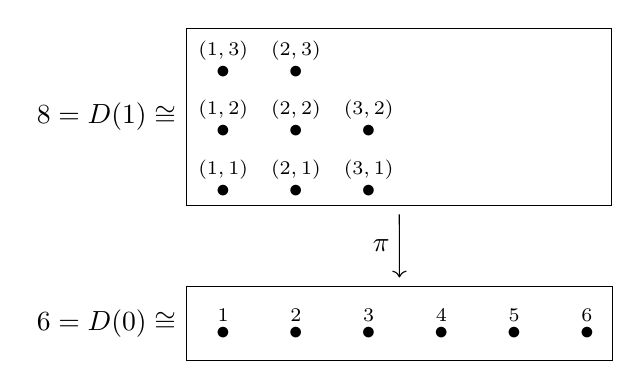
\begin{tikzpicture}[x=.5cm, y=.35cm, every label/.style={font=\scriptsize}, baseline=(f)]
	\node[label={[above=-5pt]:$1$}] (Ya) {$\bullet$};
	\node[right=1 of Ya,  label={[above=-5pt]:$2$}] (Yc) {$\bullet$};
	\node[right=1 of Yc,  label={[above=-5pt]:$3$}] (Yd) {$\bullet$};
	\node[right=1 of Yd,  label={[above=-5pt]:$4$}] (Ye) {$\bullet$};
	\node[right=1 of Ye,  label={[above=-5pt]:$5$}] (Yf) {$\bullet$};
	\node[right=1 of Yf,  label={[above=-5pt]:$6$}] (Yg) {$\bullet$};
	\node[draw, inner ysep=4pt, fit={($(Ya)+(-1em,3ex)$) (Yg)}] (Y) {};
	\node[left=0 of Y] (Ylab) {$6=D(0)\cong$};
%
  \node[above=4 of Ya, label={[above=-5pt]:$(1,1)$}] (X11) {$\bullet$};
  \node[above=1 of X11, label={[above=-5pt]:$(1,2)$}] (X12) {$\bullet$};
  \node[above=1 of X12, label={[above=-5pt]:$(1,3)$}] (X13) {$\bullet$};
%
  \node[above=4 of Yc, label={[above=-5pt]:$(2,1)$}] (X31) {$\bullet$};
  \node[above=1 of X31, label={[above=-5pt]:$(2,2)$}] (X32) {$\bullet$};
  \node[above=1 of X32, label={[above=-5pt]:$(2,3)$}] (X33) {$\bullet$};
%
  \node[above=4 of Yd, label={[above=-5pt]:$(3,1)$}] (X41) {$\bullet$};
  \node[above=1 of X41, label={[above=-5pt]:$(3,2)$}] (X42) {$\bullet$};
  \node [above=4 of Yg] (xend) {};
	\node[draw, inner ysep=3pt, fit={($(X13)+(-1em,3ex)$) ($(xend)+(.4,0)$)}] (X) {};
	\node[left=0 of X] {$8=D(1)\cong$};
%
	\draw[->, shorten <=3pt, shorten >=3pt] (X) to node[left] (f) {$\pi$} (Y);
\end{tikzpicture}
\end{equation}
\end{example}

We can think of a function $\pi\colon s\to t$, e.g.\ that shown in \eqref{eqn.bundle}, as a \emph{bundle} of fibers $\pi\inv(i)$, one for each element $`i'\in t$. In \cref{def.sheaves_bundles} we define two different notions of morphism between them. We will see in \cref{thm.equivs} that they correspond to morphisms in the categories $\poly$ and $\dir$.

For any function $\pi'\colon s'\to t'$ and function $f\colon t\to t'$, denote by $f^*(\pi')$ the pullback function as shown
\[
\begin{tikzcd}
	s\times_{t'}s'\ar[r]\ar[d, "f^*(\pi')"']&
	s'\ar[d, "\pi'"]\\
	t\ar[r, "f"']&
	t'\ar[ul, phantom, very near end, "\lrcorner"]
\end{tikzcd}
\]

\begin{definition}\label{def.sheaves_bundles}
Let $\pi\colon s\to t$ and $\pi'\colon s'\to t'$ be functions between finite sets.
\begin{itemize}
	\item a \emph{bundle morphism} consists of a pair $(f,f_\sharp)$ where $f\colon t\to t'$ is a function and $f_\sharp\colon \pi\to f^*(\pi')$ is a morphism in the slice category over $t$;
	\item a \emph{container morphism} consists of a pair $(f,f^\sharp)$ where $f\colon t\to t'$ is a function and $f^\sharp\colon f^*(\pi')\to \pi$ is a morphism in the slice category over $t$.
\end{itemize}

We say a bundle morphism $(f, f_\sharp)$ (resp. a container morphism $(f, f^{\sharp})$) is \emph{cartesian} if $f_{\sharp}$ (resp. $f^{\sharp})$ is an isomorphism.
%\begin{equation}\label{fig.bund_cont_maps}
%\begin{tabular}{ccc}
%$(f,f_\sharp)\in\bun(\pi,\pi')$&~\qquad~&
%$(f,f^\sharp)\in\cont(\pi,\pi')$\\
%\begin{tikzcd}[ampersand replacement=\&]
%s\ar[dr, bend right=40pt, "\pi"']\&[-5pt]
%t\times_{t'}s'\ar[r]\ar[d, "f^*\pi'"']\ar[from=l, "f_\sharp"]\&
%s'\ar[d, "\pi'"]\\\&
%t\ar[r, "f"']\&
%t'\ar[ul, phantom, very near end, "\lrcorner"]
%\end{tikzcd}
%&&
%\begin{tikzcd}[ampersand replacement=\&]
%s\ar[dr, bend right=40pt, "\pi"']\&[-5pt]
%t\times_{t'}s'\ar[r]\ar[d, "f^*\pi'"']\ar[l, "f^\sharp"']\&
%s'\ar[d, "\pi'"]\\\&
%t\ar[r, "f"']\&
%t'\ar[ul, phantom, very near end, "\lrcorner"]
%\end{tikzcd}
%\end{tabular}
%\end{equation}

\begin{figure}
\[
  \begin{tikzcd}
  s\ar[dr, bend right=40pt, "\pi"']&[-5pt]
  t\times_{t'}s'\ar[r]\ar[d, "f^*\pi'"']\ar[from=l, "f_\sharp"]&
  s'\ar[d, "\pi'"]\\&
  t\ar[r, "f"']&
  t'\ar[ul, phantom, very near end, "\lrcorner"]
  \end{tikzcd}
  \hspace{.75in}
  \begin{tikzcd}
  s\ar[dr, bend right=40pt, "\pi"']&[-5pt]
  t\times_{t'}s'\ar[r]\ar[d, "f^*\pi'"']\ar[l, "f^\sharp"']&
  s'\ar[d, "\pi'"]\\&
  t\ar[r, "f"']&
  t'\ar[ul, phantom, very near end, "\lrcorner"]
  \end{tikzcd}
\]
\caption{The categories $\bun$ and $\cont$ have the same objects, functions $\pi\colon s\to t$. Here a morphism $(f,f_\sharp)\colon \pi\to \pi'$ in $\bun$ and a morphism $(f,f^\sharp)\colon \pi\to\pi'$ in $\cont$ are shown.
}
\label{fig.bund_cont_maps}
\end{figure}
Define $\bun$ (resp.\ $\cont$) to be the category for which an object is a function between finite sets and a morphism is a bundle morphism (resp.\ container morphism); see \cref{fig.bund_cont_maps}. Denote by $\bun_{\text{cart}}$ (res. $\cont_{\text{cart}}$) the subcategory of cartesian bundle morphisms.
\end{definition}

One may note that $\bun$ is the Grothendieck construction of the self-indexing $\fin_{/(-)} \colon \fin\op \to \smcat$, while $\cont$ is the Grothendieck construction of its point-wise opposite $(\fin_{/(-)})\op \colon \fin\op \to \smcat$.

 The name \emph{container} comes from the work of Abbot, Altenkirch, and Ghani \cites{AAG:Containers.In.Proceedings}{AAG:Containers}{A:Containers.Thesis} (see Remark 2.18 in \cite{GK:Polynomial.Functors} for a discussion of the precise relationship between the notion of container and the notion of polynomial and polynomial functor).

\begin{remark}\label{rem.dir_fin2}
By the universal property of pullbacks, $\bun\simeq\fin^{\to}$ is equivalent (in fact isomorphic) to the category of morphisms and commuting squares in $\fin$. Furthermore, $\bun_{\text{cart}}$ is equivalent to the category of morphisms and pullback squares in $\fin$, and $\bun_{\text{cart}} \simeq \cont_{\text{cart}}$ (as in both cases a cartesian morphism $(f, f_{\sharp})$ or $(f, f^{\sharp})$ is determined by $f$ alone).
\end{remark}

\begin{remark}
We can think of a function between finite sets $\pi : E \to B$ as the categorification of a \emph{Young diagram}. A Young diagram consists of $k$ natural numbers $n_k \geq n_{k-1} \geq \cdots \geq n_1 > 0$; the number $k$ is the number of rows and $n_i$ is the number of boxes in row $i$. Here is a Young diagram corresponding to \cref{eqn.bundle} (but ignoring the constant term, which is the number of empty rows):
\[
\ydiagram{3, 3, 2}
\]

If we allow for empty rows, then we can read a function $\pi : E \to B$ as a Young diagram in the following way:
\begin{itemize}
    \item $B$ is the set of rows.
    \item $E$ is the set of pairs of a row and a box in that row.
    \item $\pi : E \to B$ is the projection which sends each pair of a box and a row to that row.
\end{itemize}
Thinking of maps $\pi : E \to B$ in this way, we can see $\bun$ as the category of Young diagrams with functions covariant in the rows and boxes, and $\cont$ as the category of Young diagrams with functions covariant in the rows but contravariant in the boxes. The category $\bun_{\text{cart}}$ (equivalently $\cont_{\text{cart}}$) is the category of functions of rows that preserve the number of boxes in each row (though it may permute the boxes within a row).
\end{remark}

 Next we show that $\bun\simeq\dir$ is also equivalent to the category of Dirichlet functors, from \cref{def.poly_dir}. Recall that a natural transformation is called \emph{cartesian} if its naturality squares are pullbacks.

\begin{theorem}\label{thm.equivs}
We have equivalences of categories
\[
\poly\simeq\cont
\qqand
\dir\simeq\bun.
\]
In particular, this gives an equivalence $\poly_{\text{cart}} \simeq \dir_{\text{cart}}$ of the category of polynomial functors and cartesian natural transformations and the category of Dirichlet functors and cartesian natural transformations.
\end{theorem}
\begin{proof}
The functors $P_-\colon\cont\to\poly$ and $D_-\colon\bun\to\dir$ are defined on each object, i.e.\ function $\pi\colon s\to t$, by the formula $\pi\mapsto P_\pi$ and $\pi\mapsto D_\pi\coloneqq\overline{P_\pi}$ as in \cref{prop.poly_function}. For each $1\leq i\leq t$, denote the fiber of $\pi$ over $i$ by $k_i\coloneqq\pi\inv(i)$.

For any finite set $X$, consider the unique map $X!\colon X\to 1$. Applying $P_-$ and $D_-$ to it, we obtain the corresponding representable: $P_{X!}\cong\yon^X$ and $D_{X!}\cong X^\yon$. We next check that there are natural isomorphisms
 \begin{gather}\nonumber
  \poly(P_{X!},P_\pi)\cong 
  P_\pi(X)=
  \sum_{}X^{k_i}\cong
  \cont(X!, \pi),
  \\\label{eqn.dir_bund}
  \dir(D_{X!}, D_\pi)\cong 
  D_\pi(X)=
  \sum_{i=1}^{t}(k_i)^X\cong
  \bun(X!, \pi).
\end{gather}
In both lines, the first isomorphism is the Yoneda lemma and the second is a computation using \cref{def.sheaves_bundles} (see \cref{fig.bund_cont_maps}). Thus we define $P_-$ on morphisms by sending $f\colon\pi\to\pi'$ in $\cont$ to the ``compose-with-$f$'' natural transformation, i.e.\ having $X$-component $\cont(X!,f)\colon\cont(X!,\pi)\to\cont(X!,\pi')$, which is clearly natural in $X$. We define $D_-$ on morphisms similarly: for $f$ in $\bun$, use the natural transformation $\bun(-!,f)$.

By definition, every object in $\poly$ and $\dir$ is a coproduct of representables, so to prove that we have the desired equivalences, one first checks that coproducts in $\cont$ and $\bun$ are taken pointwise:
\[
(\pi\colon s\to t)+(\pi'\colon s'\to t')\cong(\pi+\pi')\colon (s+s')\to (t+t'),
\]
and then that $P_{\pi+\pi'}=P_\pi+P_{\pi'}$ and $D_{\pi+\pi'}=D_\pi+D_{\pi'}$; see \cref{rem.products_coproducts}.

By \cref{rem.dir_fin2}, we know that $\bun_{\text{cart}} \simeq \cont_{\text{cart}}$, and we have just established the equivalences $\poly \simeq \cont$ and $\dir \simeq \bun$. It thus remains to check that the latter equivalences identify cartesian natural transformations in $\poly$ with cartesian morphisms in $\cont$, and similarly for $\dir$ and $\bun$. For polynomial functors, we may refer to \cite[Section 2]{GK:Polynomial.Functors}.

Turning to Dirichlet functors, we want to show that for any $f\colon D\to D'$ the square
\begin{equation}\label{eqn.cart1}
\begin{tikzcd}
	D(1)\ar[r, "f_1"]\ar[d, "\pi"']&
	D'(1)\ar[d, "\pi'"]\\
	D(0)\ar[r, "f_0"']&
	D'(0)
\end{tikzcd}
\end{equation}
is a pullback in $\smset$ iff for all functions $g\colon X\to X'$, the naturality square
\begin{equation}\label{eqn.cart2}
\begin{tikzcd}
  D(X')\ar[r, "f_{X'}"]\ar[d, "D(g)"']&
  D'(X')\ar[d, "D'(g)"]\\
  D(X)\ar[r, "f_X"']&
  D'(X)
\end{tikzcd}
\end{equation}
is a pullback in $\smset$; we will freely use the natural isomorphism $D_\pi(X)\cong\bun(X!,\pi)$ from \cref{eqn.dir_bund}. The square in \cref{eqn.cart1} is a special case of that in \cref{eqn.cart2}, namely for $g\coloneqq 0!$ the unique function $0\to 1$; this establishes the only-if direction.

To complete the proof, suppose that \cref{eqn.cart1} is a pullback, take an arbitrary $g\colon X\to X'$, and suppose given a commutative solid-arrow diagram as shown:
\[
\begin{tikzcd}[sep=small]
  X\ar[rr, "g"]\ar[dd]\ar[rd]&&
  X'\ar[dr]\ar[dd]\ar[dl, dotted]\\&
  D(1)\ar[rr, crossing over]&&
  D'(1)\ar[dd]\\
  1\ar[dr]\ar[rr, equal]&&
  1\ar[dr]\ar[dl, dotted]\\&
  D(0)\ar[from=uu, crossing over]\ar[rr]&&
  D'(0)
\end{tikzcd}
\]
We can interpret the statement that \cref{eqn.cart2} is a pullback as saying that there are unique dotted arrows making the diagram commute, since $DX \cong \bun(X!,  D0!)$ and similarly for the other corners of the square in \cref{eqn.cart2}. So, we need to show that if the front face is a pullback, then there are unique diagonal dotted arrows as shown, making the diagram commute. This follows quickly from the universal property of the pullback.
%
%
%
%
%
%We first note that a natural transformation $\phi : D \to D'$ between Dirichlet functors is cartesian if and only if the naturality square induced by $!X\colon 0 \to X$
%
%\begin{equation}\label{diagram:nat.square}
%\begin{tikzcd}
%DX \arrow[r, "\phi_X"] \arrow[d, "D(!X)"'] & 
%D'X \arrow[d, "D'(!X)"] \\
%D0 \arrow[r, "\phi_0"'] & D'0
%\end{tikzcd}
%\end{equation}
%is a pullback for all $X$, by the pullback pasting lemma. Now, the associated bundle morphism $\phi_{1!}$ associated to $\phi$ is the particular naturality square
%\begin{equation}\label{diagram:bundle.morphism}
%\begin{tikzcd}
%D1 \arrow[r, "\phi_1"] \arrow[d, "D(!1)"'] & D'1 \arrow[d, "D'(!1)"] \\
%D0 \arrow[r, "\phi_0"'] & D'0
%\end{tikzcd}
%\end{equation}
%
%So, if $\phi$ is cartesian then the associated bundle morphism is. We now assume the associated bundle morphism \cref{diagram:bundle.morphism} is cartesian, and show that $\phi$ is cartesian by showing that \cref{diagram:nat.square} is a pullback for each $X$.
%
%Recall that 
%\[
%DX \cong 
%\bun\left(
%	\begin{tikzcd}[sep=small] 
%		X \arrow[d] \\ 
%		1 
%	\end{tikzcd}\,,\; 
%	\begin{tikzcd}[sep=small] 
%	D(1) \arrow[d] \\ 
%	D(0) 
%	\end{tikzcd} 
%\right) = \bun(X!, D),
%\]
%and the map $D(!X)\colon DX \to D0$ is equivalent under this isomorphism to the map that returns just the bottom component of a bundle morphism. Therefore, we can equivalently write \cref{diagram:nat.square} as
%\begin{equation}
%    \begin{tikzcd}[column sep=large]
%    \bun(X!, D) \arrow[d] \arrow[r, "\phi \circ -"] & \bun(X!, D') \arrow[d] \\
%    D0 \arrow[r] & D'0
%    \end{tikzcd}
%\end{equation}
%This will be a pullback if for all $z \in D0$, the induced map on the fibers of the vertical functions in this square over $z$ is bijection. This map is the map
%\[
%\zeta : \left\{ \begin{tikzcd}
%X \arrow[r, dashed] \arrow[d] & D1 \arrow[d] \\
%1 \arrow[r, "z"'] & D0
%\end{tikzcd} \right\} \to \left\{\begin{tikzcd}
%X \arrow[r, dashed] \arrow[d] & D'1 \arrow[d] \\
%1 \arrow[r, "\phi_0 z"'] & D'0
%\end{tikzcd} \right\}
%\]
%given by post-composition with \eqref{diagram:bundle.morphism}, which we have assumed is a pullback square. The universal property of this pullback then says that the map $\zeta$ is a bijection.
\end{proof}

\begin{corollary}\label{cor.dir_topos}
$\dir$ is an elementary topos.
\end{corollary}
\begin{proof}
For any finite category $C$, the functor category $\fin^C$ is an elementary topos. The result now follows from \cref{rem.dir_fin2,thm.equivs}, noting that $\dir \simeq \fin^{\to}$.
\end{proof}

\begin{theorem}
A functor $D : \finset\op \to \finset$ is a Dirichlet polynomial if and only if it preserves connected limits, or equivalently wide pullbacks.
\end{theorem}
\begin{proof}
If $D(X) = \sum_{b \in B} E_b^X$ is a Dirichlet polynomial corresponding to the map $\pi : E \to B$, then
\begin{align*}
    D(\colim X_i) &= \sum_{b \in B} E_b^{\colim X_i} \\
    &\cong \sum_{b \in B} \lim E_b^{X_i} \\
    &\cong \lim \sum_{b \in B} E_b^{X_i} \\
    &= \lim D(X_i)
\end{align*}
for any connected colimit, since connected limits commute with sums. On the other hand, suppose $D$ sends connected colimits to connected limits -- in particular, it sends wide pushouts to wide pullbacks. Every finite set $X$ can be expressed as the wide pushout
\[
% https://tikzcd.yichuanshen.de/#N4Igdg9gJgpgziAXAbVABwnAlgFyxMJZABgBoBGAXVJADcBDAGwFcYkRyQBfU9TXfIRTkK1Ok1btOPPtjwEiAZlE0GLNog7deIDHMFEALCvHqp22QIUoATCbWTNAHScBjKBBwIZu-vKHIdjZiDhogxBa++taBpMQhEmEAGtxiMFAA5vBEoABmAE4QALZIAKw0OBBIxD4FxWUVVYjktYUliOUglUg2rfUdjUiKfe1kXU0AbCNIIuNIUzp17XZziAt5bUODa1yUXEA
\begin{tikzcd}
              &              & X                                               &              &               \\
1 \arrow[rru] & 1 \arrow[ru] & \cdots                                          & 1 \arrow[lu] & 1 \arrow[llu] \\
              &              & 0 \arrow[llu] \arrow[lu] \arrow[ru] \arrow[rru] &              &              
\end{tikzcd}
\]
of its elements. Therefore, we have the following limit diagram:
\[
% https://tikzcd.yichuanshen.de/#N4Igdg9gJgpgziAXAbVABwnAlgFyxMJZABgBoBGAXVJADcBDAGwFcYkQARACnIEoQAvqXSZc+QinIVqdJq3bc+g4SAzY8BIgCZpNBizaIQAHWMBjKBBwIhI9eKIBmXbIMKe-W6tEaJyACwu+vJGip4qamKaKDpaMsGGnFzE4XZRfjrE8XKJ3AAanjIwUADm8ESgAGYAThAAtkgAbDQ4EEjEXjX1TS1tiOSdtQ2IzSCtSI6D3SO9SP5Tw2RjfQCsC0hSy0hrKl3DzluIO1VDc7NHApQCQA
\begin{tikzcd}
                 &                 & D(X) \arrow[lld] \arrow[ld] \arrow[rd] \arrow[rrd] &                 &                  \\
D(1) \arrow[rrd] & D(1) \arrow[rd] & \cdots                                             & D(1) \arrow[ld] & D(1) \arrow[lld] \\
                 &                 & D(0)                                               &                 &                 
\end{tikzcd}
\]
That is, an element of $D(X)$ is a family of elements $a_x \in D(1)$ for each $x \in X$, such that the $D0!(a_x)$ are all equal in $D(0)$. In other words, 
$$D(X) \cong \bun(X!, D0!)$$
which is to say $D$ is the Dirichlet polynomial associated to the bundle $D0!$.
\end{proof}


As we mentioned in the introduction, this all goes through smoothly when one drops all finiteness conditions. The general topos of Dirichlet functors is the category of (arbitrary) sums of representables $\smset\op \to \smset$, and this is equivalent to the arrow category $\smset^{\to}$ and so is itself a topos.

\section*{Acknowledgments}

Thanks to Joachim Kock for helpful comments on an early draft of this note.

%\chapter{The $\poly-\dir$ double category $\ff$}
%
%There is a double category $\ff$ whose objects are functions between finite sets, whose vertical category is $\poly$, whose horizontal category is isomorphic to $\bun$. This double category shows up in the theory of mode-dependent dynamical systems, though we save this for future work.
%
%The double category $\ff$ will be thin, meaning that for every square there is at most one 2-cell filler. Squares (with or without filler) can be drawn as \emph{bevelled squares}:
%\[
%\begin{tikzcd}[sep=large]
%&[-35pt]
%\overline{P}\ar[r, "f"]&
%\overline{Q}\\[-25pt]
%P\ar[d, "g"']\arrow[ur, no head]&&&[-35pt]\ar[ul, no head]\ar[d, "h"]
%Q\\
%P'\ar[dr, no head]&&&
%Q'\ar[dl, no head]\\[-25pt]&
%\overline{P}'\ar[r, "f'"']&
%\overline{Q}'
%\end{tikzcd}
%\]
%where $g,h$ are in $\poly$ and $f,f'$ are in $\dir$, and where the unlabeled line segments are just tracking Dirchlet transforms. Thus to define $\ff$, it remains to give the conditions for when a filler exists for $(f,f',g,h)$; there will be two.
%
%Suppose first that $P=\yon^m$ is a pure power, i.e.\ $P(1)=1$; this is the case iff its Dirichlet transform $\overline{P}=m^\yon$ is a pure exponential $D(0)=1$. In that case $g$ picks out an element $g(1)\in P'(1)=\ol{P}'(0)$ and $f$ picks out an element $f(1)\in \ol{Q}(0)=Q(1)$. Let $m'$ be the finite set corresponding to the exponent on $g(1)$ and let $n$ be the finite set corresponding to the base on $f(1)$
%\[
%  \yon^{m'}\coloneqq P'\times_{P(1)}g(1)
%  \qqand
%  n^\yon\coloneqq\ol{Q}\times_{\ol{Q}(0)}f(1)
%\]
%Then $f'$ picks out an element $f'(g(1))\in\ol{Q}'(0)=Q'(1)$ and $h$ picks out an element $h(f(1))\in Q'(1)=\ol{Q}'(0)$. The first condition is that $h(f(1))=f'(g(1))$. We may then define $n'$ to be the corresponding finite set, so that
%\[
%  \yon^{n'}= Q'\times_{Q'(1)}f'(g(1))
%  \qqand
%  (n')^\yon=\ol{Q}'\times_{\ol{Q}'(0)}h(f(1))
%\]
%By \cref{fig.bund_cont_maps} we then obtain four maps
%\begin{align*}
%	g^\sharp&\colon\yon^m\to\yon^{m'}&
%	f_\sharp&\colon m^\yon\to n^\yon\\
%	f'_\sharp&\colon(m')^\yon\to(n')^\yon&
%	h^\sharp&\colon\yon^{n}\to\yon^{n'}
%\end{align*}
%and by the Yoneda lemma, these induce composable functions
%\[
%  m'\To{g^\sharp} m\To{f_\sharp} n
%  \qqand
%  m'\To{f'_\sharp} n'\To{h^\sharp} n
%\]
%The second condition is that these are the same function $m'\to n$. 
%
%In general, $P$ may not be a pure power, but it is a coproduct over $i\in P(1)$ of pure powers $\yon^{p_i}$. We say that a beveled square has a filler iff the above two conditions hold for each summand.
%
%It is easy to check that we indeed have a double category.
%\begin{theorem}
%There is a thin double category whose objects are functions $\pi\colon s\to t$, whose vertical category is $\poly\cong\cont$, whose horizontal category is $\dir\cong\bun$, and for which 2-cells are defined as above.
%\end{theorem}

\iffalse
\section{Analytic Functors and Dirichlet Series}

Given a combinatorial species $A : \fin^{\cong} \to \smset$, its
\emph{Cauchy generating functor} $X \mapsto \sum_{n : \fin} A_n \times X^n/n!$
is the left Kan extension of $A$ along the inclusion $\fin^{\cong}
\hookrightarrow \smset$, and the \emph{Dirichlet generating functor} $S \mapsto
\sum_{n : \fin} A_n n^S/n!$ is the left Kan extension of $A$ along the
inclusion $\fin^{\cong} \hookrightarrow \smset^{\text{op}}$. These give
functors
\[
  \begin{tikzcd}
    & \textbf{CombSpecies} \arrow[dr, "|\cdot|_{\dir}"] \arrow[dl, "|\cdot|_{\poly}"']& \\
    \poly & & \dir
  \end{tikzcd}
\]

The Cauchy product $\otimes_{\poly}$ of combinatorial species is given by Day
convolution from $+ : \fin^{\cong} \times \fin^{\cong}$, and
$|\cdot|_{\poly}$ sends $\otimes_{\poly}$ to the cartesian product in $\poly$. On the
other hand, the Dirichlet product $\otimes_{\dir}$ of combinatorial species is
given by Day convolution from $\times : \fin^{\cong} \times
\fin^{\cong}$, and this is sent by $|\cdot|_{\dir}$ to the cartesian
product in $\dir$. This gives us an interpretation of the generating \emph{functors}
associated to a species in which sum is coproduct and product is cartesian
product -- the difference between the Cauchy generating functor and the
Dirichlet generating functor is that the latter is contravariant.

Dirichlet series also form a topos.
\begin{theorem}
The category $\dir_{\infty}$ of \emph{Dirichlet series} -- functors $\fin\op \to \smset$ which are sums of representables -- \emph{almost} form an elementary topos.
\end{theorem}
\begin{proof}
As for Diriclet polynomials, for any Dirichlet series $D$ we have a map $\pi_D : D(1) \to D(0)$; however, $D(1)$ and $D(0)$ are no longer finite sets. It is the case, however, that $\pi_D$ has finite fibers. This gives us a functor $\dir_{\infty} \to \bun_f$ from Dirichlet series to the full subcategory $\bun_f \hookrightarrow \smset^{\to}$ of the arrow category of $\smset$ consisting of those maps with finite fibers. We will show that this map is an equivalence, and that $\bun_f$ is an \emph{almost} elementary topos.
\end{proof}
\fi


\printbibliography

\end{document}